In this chapter, we will define a tuple $(\Phi,\alpha,\beta,\gamma)$ constituting a logic translation from FOLEQ to HOL. The four components will be defined individually. Moreover, each of them has two components, one dealing with signatures, one dealing with signature morphisms:

\section{The Object Dimension}

\begin{definition}[Signature Translation]\label{def:folhol:syn}
Given a FOLEQ signature $\Sigma=(\Sigma_f,\Sigma_p,\arit)$, the HOL signature $\Phi(\Sigma)$ contains the following declarations:
  \begin{itemize}
   \item $\iota:\TYPE$
   \item $f:\underbrace{\iota \arr\ldots\arr\iota}_n\arr\iota$ for every $f\in\Sigma_f$ with $\arit(f)=n$
   \item $p:\underbrace{\iota \arr\ldots\arr\iota}_n\arr o$ for every $p\in\Sigma_p$ with $\arit(p)=n$
  \end{itemize}
\end{definition}
\medskip

\begin{definition}[Expression Translation]\label{def:folhol:sen}
Given $\isterm{\Sigma}{\Gamma}{t}$ or $\isform{\Sigma}{\Gamma}{F}$, we define $\alpha_\Sigma(t)$ and $\alpha_\Sigma(F)$ by induction of $\Gamma$, $t$, and $F$. We omit the details.
\end{definition}
\medskip

\begin{definition}[Judgment and Proof Translation]\label{def:folhol:pt}
Given a $\Sigma$-judgment $J\in\Pf^{\FOLEQ}(\Sigma)$ (see Def.~\ref{def:fol:pf}), the $\Phi(\Sigma)$-judgment $\gamma_\Sigma(J)$ is defined as follows:
\[
\cas{
  \oftype{\Phi(\Sigma)}{x_1:\iota,\ldots,x_n:\iota}{\alpha_\Sigma(t)}{\iota}
    \mifc J \; = \; \isterm{\Sigma}{x_1,\ldots,x_n}{F} \\
  \oftype{\Phi(\Sigma)}{x_1:\iota,\ldots,x_n:\iota}{\alpha_\Sigma(F)}{o}
    \mifc J \; = \; \isform{\Sigma}{x_1,\ldots,x_n}{F} \\
  \iscons{\Phi(\Sigma)}{\alpha_\Sigma(F_1),\ldots,\alpha_\Sigma(F_n)}{x_1:\iota,\ldots,x_n:\iota}{\alpha_\Sigma(F)}
    \mifc J \; = \; \iscons{\Sigma}{F_1,\ldots,F_m}{x_1,\ldots,x_n}{F}
}\]

Given a $\Sigma$-proof $p$ of a judgment $J$ using assumptions $J_1,\ldots,J_m$, the $\Phi(\Sigma)$-proof $\gamma_\Sigma(p)$ of $\gamma_\Sigma(J)$ using assumptions $\gamma_\Sigma(J_1)$, \ldots, $\gamma_\Sigma(J_m)$ is obtained by induction of $p$. We omit the details.
\end{definition}

\begin{remark}\label{rem:folhol:pt}
Note that the second part of this definition includes a substantial theorem: By mapping every $\Sigma$-proof of $J$ to a $\Phi(\Sigma)$-proof of $\gamma_\Sigma(J)$, we show that all proofs are translated. In particular, if $J$ is provable over $\Sigma$, then so is $\gamma_\Sigma(J)$ over $\Pf^{\HOL}(\Phi(\Sigma))$.
\end{remark}
\medskip

\begin{definition}[Model \advanced{and Model Morphism} Translation]\label{rem:folhol:mt}
Given a $\Sigma$-model $I\in\Mod^{\FOLEQ}(\Phi(\Sigma))$, the $\Sigma$-model $\beta_\Sigma(I)$ is defined as follows:
\footnote{homework}

\advanced{
Given a $\Sigma$-model morphism $m:I\arr I'$ in $\Mod^{\FOLEQ}(\Phi(\Sigma))$, the $\Sigma$-model morphism $\beta_\Sigma(m):\beta_\Sigma(I)\arr\beta_\Sigma(I')$ is defined as follows:
}
\end{definition}

\section{The Morphism Dimension}

\footnote{This whole section can be skipped.}

\begin{definition}[Signature Morphism Translation]\label{def:folhol:synmor}
Given a FOLEQ signature morphism $\sigma:\Sigma\arr\Sigma'$, the HOL signature morphism $\Phi(\sigma):\Phi(\Sigma)\arr\Phi(\Sigma')$ maps as follows:
  \begin{itemize}
   \item $\iota\mapsto \iota$
   \item $f\mapsto \lam{x_1}{\iota}\ldots\lam{x_n}{\iota}\sigma(f)$ for every $f\in\Sigma_f$ with $\arit(f)=n$
   \item $p\mapsto \lam{x_1}{\iota}\ldots\lam{x_n}{\iota}\sigma(p)$ for every $p\in\Sigma_p$ with $\arit(p)=n$
  \end{itemize}
\end{definition}
Recall that Def.~\ref{def:fol:sigmorph} makes $\sigma(f)$ and $\sigma(p)$ expressions with free variables $x_1,\ldots,x_n$. Those can now be properly bound because we have $\lambda$-abstraction in HOL.
\medskip

Now consider a FOLEQ-signature morphism $\sigma:\Sigma\arr\Sigma'$ and an expression $E$ over $\Sigma$. There are now two ways to translate $E$ to an expression over $\Phi(\Sigma')$, depending on whether we first translate along $\sigma$ or first along $\alpha$:

\begin{center}
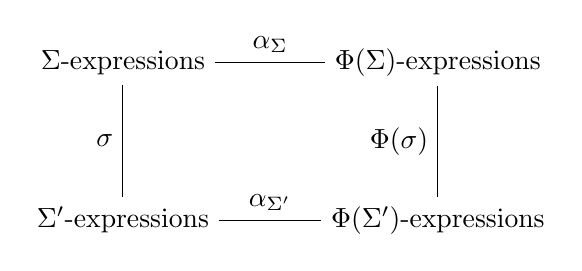
\begin{tikzpicture}[scale=2]
\node (S) at (0,1) {$\Sigma$-expressions};
\node (S') at (0,0) {$\Sigma'$-expressions};
\node (P) at (2,1) {$\Phi(\Sigma)$-expressions};
\node (P') at (2,0) {$\Phi(\Sigma')$-expressions};
\draw[-\arrowtip] (S) -- node[left]{$\ov{\sigma}$} (S');
\draw[-\arrowtip] (S) -- node[above]{$\alpha_\Sigma$} (P);
\draw[-\arrowtip] (P) -- node[left]{$\ov{\Phi(\sigma)}$} (P');
\draw[-\arrowtip] (S') -- node[above]{$\alpha_{\Sigma'}$} (P');
\end{tikzpicture}
\end{center}

In particular, recalling that $\Sen(\Sigma)$ contains those expressions that are sentences and that $\Sen(\sigma)$ is the restriction of $\ov{\sigma}$ to $\Sen(\Sigma)$:

\begin{center}
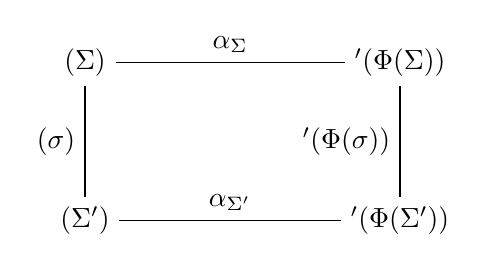
\begin{tikzpicture}[scale=2]
\node (S) at (0,1) {$\Sen(\Sigma)$};
\node (S') at (0,0) {$\Sen(\Sigma')$};
\node (P) at (2,1) {$\Sen'(\Phi(\Sigma))$};
\node (P') at (2,0) {$\Sen'(\Phi(\Sigma'))$};
\draw[-\arrowtip] (S) -- node[left]{$\Sen(\sigma)$} (S');
\draw[-\arrowtip] (S) -- node[above]{$\alpha_\Sigma$} (P);
\draw[-\arrowtip] (P) -- node[left]{$\Sen'(\Phi(\sigma))$} (P');
\draw[-\arrowtip] (S') -- node[above]{$\alpha_{\Sigma'}$} (P');
\end{tikzpicture}
\end{center}

It turns out, it these two are equal:

\begin{lemma}[Commutativity of $\Phi$ and $\alpha$]\label{lem:folhol:senmor}
For all $\sigma:\Sigma\arr\Sigma$ in $\Sig^{\FOLEQ}$, we have $\�{\alpha_\Sigma}{\ov{\Phi(\sigma)}}=\�{\ov{\sigma}}{\alpha_{\Sigma'}}$.
\end{lemma}
\medskip

A similar situation arises for the judgment and proof translation:

\begin{center}
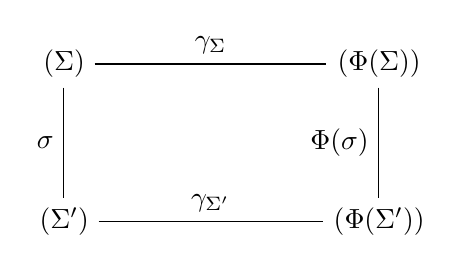
\begin{tikzpicture}[scale=2]
\node (S) at (0,1) {$\Pf^{\FOLEQ}(\Sigma)$};
\node (S') at (0,0) {$\Pf^{\FOLEQ}(\Sigma')$};
\node (P) at (2,1) {$\Pf^{\HOL}(\Phi(\Sigma))$};
\node (P') at (2,0) {$\Pf^{\HOL}(\Phi(\Sigma'))$};
\draw[-\arrowtip] (S) -- node[left]{$\ov{\sigma}$} (S');
\draw[-\arrowtip] (S) -- node[above]{$\gamma_\Sigma$} (P);
\draw[-\arrowtip] (P) -- node[left]{$\ov{\Phi(\sigma)}$} (P');
\draw[-\arrowtip] (S') -- node[above]{$\gamma_{\Sigma'}$} (P');
\end{tikzpicture}
\end{center}

Again it turns out, both are equal:

\begin{lemma}[Commutativity of $\Phi$ and $\gamma$]\label{def:folhol:ptmor}
For all $\sigma:\Sigma\arr\Sigma$ in $\Sig^{\FOLEQ}$, we have $\�{\gamma_\Sigma}{\ov{\Phi(\sigma)}}=\�{\ov{\sigma}}{\gamma_{\Sigma'}}$ both for judgments and for proofs.
\end{lemma}
\medskip

Finally, the corresponding situation -- but with reversed directions -- arises for the model translation:

\begin{center}
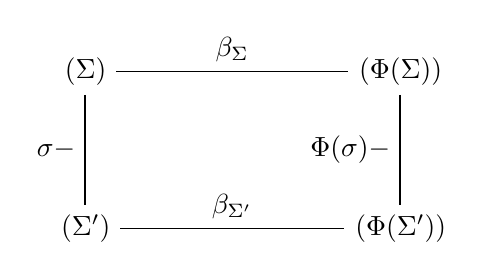
\begin{tikzpicture}[scale=2]
\node (S) at (0,1) {$\Mod^{\FOLEQ}(\Sigma)$};
\node (S') at (0,0) {$\Mod^{\FOLEQ}(\Sigma')$};
\node (P) at (2,1) {$\Mod^{\HOL}(\Phi(\Sigma))$};
\node (P') at (2,0) {$\Mod^{\HOL}(\Phi(\Sigma'))$};
\draw[\arrowtip-] (S) -- node[left]{$\reduce{\sigma}{-}$} (S');
\draw[\arrowtip-] (S) -- node[above]{$\beta_\Sigma$} (P);
\draw[\arrowtip-] (P) -- node[left]{$\reduce{\Phi(\sigma)}{-}$} (P');
\draw[\arrowtip-] (S') -- node[above]{$\beta_{\Sigma'}$} (P');
\end{tikzpicture}
\end{center}

Again it turns out, both are equal:

\begin{lemma}[Commutativity of $\Phi$ and $\beta$]\label{def:folhol:mtmor}
For all $\sigma:\Sigma\arr\Sigma$ in $\Sig^{\FOLEQ}$, we have $\�{\reduce{\Phi(\sigma)}{-}}{\beta_\Sigma}=\�{\beta_{\Sigma'}}{\reduce{\sigma}{-}}$ both for models \advanced{and model morphisms}.
\end{lemma}
\medskip

\section{Invariants}\label{sec:folhol:inv}

%However, that alone is not worth much yet: We could simply translation all judgments to a trivially true judgment $J$ one and all proofs to some proof of $J$. That would be a useless proof theory translation that nonetheless preserves provability. We need one additional requirement: The translation should also preserve proof theoretical truth. This is the content of the lemma:

As pointed out in Rem.~\ref{rem:folhol:pt}, the existence of $\gamma$ already guarantees that provability is preserved. Moreover, we observe:

\begin{lemma}[Commutativity of $\alpha$ and $\gamma$]
For all $\Sigma\in\Sig^{\FOLEQ}$ and all $F\in\Sen^{\FOLEQ}(\Sigma)$, we have
 \[\gamma_\Sigma(\val^{\FOLEQ}_\Sigma F)\; = \;\val^{\HOL}_{\Phi(\Sigma)}(\alpha_\Sigma(F)).\]
\end{lemma}
\begin{proof}
Directly from the definitions.
\end{proof}

Now we know that the validity of FOLEQ is translated to the validity judgment of HOL. Together with the proof-preservation of $\gamma$, we obtain the central theorem:

\begin{notation}
For $\Theta\sq\Sen(\Sen(\Sigma)$, we write $\alpha_\Sigma(\Theta)$ for $\{\alpha_\Sigma(F) : F\in\Theta\}$.
\end{notation}

\begin{theorem}[Preservation of Proof-Theoretical Consequence]
For all $\FOLEQ$-theories $(\Sigma,\Theta)$ and all $F\in\Sen(\Sigma)$, if $F$ is a proof theoretical theorem of $(\Sigma,\Theta)$, then $\alpha_\Sigma(F)$ is a proof theoretical theorem of $(\Phi(\Sigma),\alpha_\Sigma(\Theta))$.
\end{theorem}
\begin{proof}
Immediate.
\end{proof}


\begin{lemma}[Commutativity of $\alpha$ and $\beta$]\label{lem:folhol:mtinv}
For all $\Sigma\in\Sig^{\FOLEQ}$ and all $F\in\Sen^{\FOLEQ}(\Sigma)$, we have
 \[\moda[\FOLEQ]{\beta_\Sigma(I)}{\Sigma}{F}\tb\miff\tb\moda[\HOL]{I}{\Phi(\Sigma)}{\alpha_\Sigma(F)} \tb\mforall M\in\Mod^{\HOL}(\Phi(\Sigma)).\]
\end{lemma}

Now we know that the satisfaction relation of FOLEQ is translated to the satisfaction relation of HOL. This yields the central theorem:
\begin{theorem}[Preservation of Model-Theoretical Consequence]
For all $\FOLEQ$-theories $(\Sigma,\Theta)$ and all $F\in\Sen(\Sigma)$, if $F$ is a model theoretical theorem of $(\Sigma,\Theta)$, then $\alpha_\Sigma(F)$ is a model theoretical theorem of $(\Phi(\Sigma),\alpha_\Sigma(\Theta))$.
\end{theorem}
\begin{proof}
Assume $I\in\Mod^{\HOL}(\Phi(\Sigma))$ and $\moda[\HOL]{I}{\Phi(\Sigma)}{\alpha_\Sigma(A)}$ for all $A\in\Theta$ (*). We need to show $\moda[\HOL]{I}{\Phi(\Sigma)}{\alpha_\Sigma(F)}$. (*) and Lem.~\ref{lem:folhol:mtinv} yield $\moda[\FOLEQ]{\beta_\Sigma(I)}{\Sigma}{A}$ for all $A\in\Theta$. Therefore, using that $F$ is a model theoretical theorem of $(\Sigma,\Theta)$, we infer $\moda[\FOLEQ]{\beta_\Sigma(I)}{\Sigma}{F}$. Using Lem.~\ref{lem:folhol:mtinv} again, we obtain the needed property.
\end{proof}


